\documentclass[a4paper,12pt]{article}

%%% Работа с русским языком
\usepackage{cmap}					% поиск в PDF
\usepackage{mathtext} 				% русские буквы в формулах
\usepackage[T2A]{fontenc}			% кодировка
\usepackage[utf8]{inputenc}			% кодировка исходного текста
\usepackage[english,russian]{babel}	% локализация и переносы

%%% Дополнительная работа с математикой
\usepackage{amsmath,amsfonts,amssymb,amsthm,mathtools} % AMS
\usepackage{icomma} % "Умная" запятая: $0,2$ --- число, $0, 2$ --- перечисление

%% Номера формул
%\mathtoolsset{showonlyrefs=true} % Показывать номера только у тех формул, на которые есть \eqref{} в тексте.
%\usepackage{leqno} % Нумерация формул слева

%% Свои команды
\DeclareMathOperator{\sgn}{\mathop{sgn}}

%% Перенос знаков в формулах (по Львовскому)
\newcommand*{\hm}[1]{#1\nobreak\discretionary{}
{\hbox{$\mathsurround=0pt #1$}}{}}

%%% Работа с картинками
\usepackage{graphicx}  % Для вставки рисунков
\graphicspath{materials}  % папки с картинками
\setlength\fboxsep{3pt} % Отступ рамки \fbox{} от рисунка
\setlength\fboxrule{1pt} % Толщина линий рамки \fbox{}
\usepackage{wrapfig} % Обтекание рисунков текстом

%%% Работа с таблицами
\usepackage{array,tabularx,tabulary,booktabs} % Дополнительная работа с таблицами
\usepackage{longtable}  % Длинные таблицы
\usepackage{multirow} % Слияние строк в таблице

%%% Теоремы
\theoremstyle{plain} % Это стиль по умолчанию, его можно не переопределять.
\newtheorem{theorem}{Теорема}[section]
\newtheorem{proposition}[theorem]{Утверждение}
 
\theoremstyle{definition} % "Определение"
\newtheorem{corollary}{Следствие}[theorem]
\newtheorem{problem}{Задача}[section]
 
\theoremstyle{remark} % "Примечание"
\newtheorem*{nonum}{Решение}

%%% Программирование
\usepackage{etoolbox} % логические операторы

%%% Страница
%\usepackage{extsizes} % Возможность сделать 14-й шрифт
\usepackage{geometry} % Простой способ задавать поля
	\geometry{top=25mm}
	\geometry{bottom=30mm}
	\geometry{left=25mm}
	\geometry{right=25mm}
 %

%%% Способ сделать тоже самое(но красивее:)
%\usepackage[margin=0.8in]{geometry}

 
\usepackage{fancyhdr} % Колонтитулы
 	\pagestyle{fancy}
 	\renewcommand{\headrulewidth}{0mm}  % Толщина линейки, отчеркивающей верхний колонтитул
 	\lfoot{}
 	\rfoot{}
 	\rhead{}
 	\chead{}
 	\lhead{ }
 	% \cfoot{Нижний в центре} % По умолчанию здесь номер страницы

\usepackage{setspace} % Интерлиньяж
%\onehalfspacing % Интерлиньяж 1.5
%\doublespacing % Интерлиньяж 2
%\singlespacing % Интерлиньяж 1

\usepackage{lastpage} % Узнать, сколько всего страниц в документе.

\usepackage{soulutf8} % Модификаторы начертания

\usepackage{hyperref}
\usepackage[usenames,dvipsnames,svgnames,table,rgb]{xcolor}
\hypersetup{				% Гиперссылки
    unicode=true,           % русские буквы в раздела PDF
    pdftitle={Заголовок},   % Заголовок
    pdfauthor={Автор},      % Автор
    pdfsubject={Тема},      % Тема
    pdfcreator={Создатель}, % Создатель
    pdfproducer={Производитель}, % Производитель
    pdfkeywords={keyword1} {key2} {key3}, % Ключевые слова
    colorlinks=true,       	% false: ссылки в рамках; true: цветные ссылки
    linkcolor=red,          % внутренние ссылки
    citecolor=green,        % на библиографию
    filecolor=magenta,      % на файлы
    urlcolor=blue           % на URL
}

%\renewcommand{\familydefault}{\sfdefault} % Начертание шрифта

\usepackage{multicol} % Несколько колонок

% Мои "дополнительные" пакеты
\usepackage{textcase} 
\usepackage{pdfpages}
\usepackage{amsmath}
\usepackage{titlesec}
\usepackage{floatrow}

\usepackage{subfig}

%% Делаем красивый header:
\fancyhead[RO]{\footnotesize{\scshape\nouppercase{~\leftmark}}}
%% Делаем красивый header END

%Делаем большой отступ между section и subsection
\titlespacing*{\section} {0pt}{3.5ex plus 1ex minus .2ex}{2.7ex plus .2ex}
\titlespacing*{\subsection} {0pt}{2.7ex plus 1ex minus .2ex}{1ex plus .2ex}


\begin{document} % конец преамбулы, начало документа

\begin{center}
	\textit{\MakeTextUppercase{федеральное государственное автономное учреждение}}
		
	\vspace{0.5ex}
	
	\textbf{ \\ \MakeTextUppercase{<<Московский Физико-технический институт>>}}
\end{center}
\vspace{13ex}
\begin{flushright}
	\noindent
	{Подкидышев Алексей}
	\\
	\textit{Студент факультета инноваций\\ и высоких технологий\\(группа 792)}
\end{flushright}
\begin{center}
	\vspace{23ex}
	\line(1,0){430}\\[4ex]
	{\LARGE\textbf{Лабораторная работа 10.1}}
	\vspace{2ex}\\
	\textbf{\large{<<Электронный парамагнитный резонанс>>}}\\[3ex]
	\line(1,0){430}\\[5ex]
	\vfill
	Долгопрудный 
	
	{\today}
\end{center}
\newpage
\renewcommand{\headrulewidth}{1pt}
	\section{Теория}
\begin{multicols}{2}
[
\subsection*{Ход Работы}
]
	Энергетический уровень электрона в присутствии магнитного поля $B$ расщепляется на два подуровня, расстояние между которыми равно:
		\begin{equation}
		    \Delta E = E_2 - E_1 = 2\mu B
		\end{equation}
		Между этими двумя уровнями возможны переходы. Они могут возбуждаться внешним высокочастотным магнитным полем подходящих характеристик.
		Резонансное значение частоты определяется из очевидного соотношения:
		\begin{equation}
		    \hbar\omega_0 = \Delta E =2\mu B
		\end{equation}
	    При переходе с нижнего на верхний уровень квант энергии поглощается, а при обратном переходе излучается квант той же частоты. Возбуждение электронных резонансных переходов электромагнитным полем с частотой $\omega_0$ носит название <<электронного парамагнитного резонанса>>
	    Сигнал ЭПР наблюдается только на неспаренных электронах образца. В работе используется образец свободного радикала ДФПГ.
\end{multicols}

 \begin{figure}[h!]
\centering
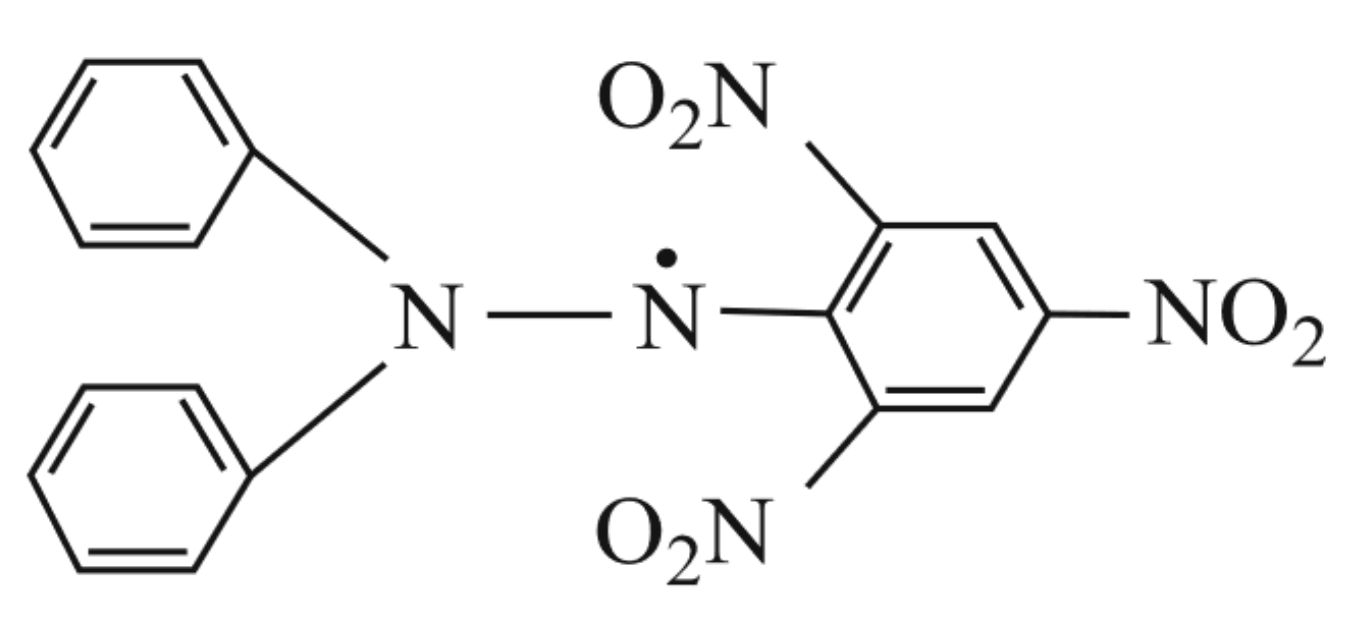
\includegraphics[width=0.7\linewidth]{dfpg.PNG}
\caption{Дифенилпикрилгидразил}
\end{figure}

\begin{multicols}{2}
    Рассмотрим основные процессы, влияющие на ширину линии ЭПР. В отсутсвие высокочастотного поля заселенность верхнего и нижнего уровней $N_u$ и $N_d$ определяется температурой и описывается формулой Больцмана.
    \begin{equation}
        \frac{N_u}{N_d} = exp\left(-\frac{\Delta E}{kT}\right)
    \end{equation}
    В присутствии резонансного поля между уровнями возникают индуцированные переходы, ведущие к тому, что заселенность верхнего уровня растет, а нижнего падает. Этот процесс ведет к нарушению соотношения Больцмана. Восстановление теплового равновесия происходит двумя способами: спин-спиновой и спин-решеточной релаксацией.
    Отличить их друг от друга можно по температурной зависимости: спин-решеточное взаимодействие быстро возрастает с температурой(числом фононов), спин-спиновое от температуры практически не зависит.
    Согласно соотношению неопределенностей:
    \begin{equation}
        \Delta\omega\tau \simeq 1
    \end{equation}
\end{multicols}
	\newpage
	\section{Установка}
        В работе требуется получить ЭПР сигнал на ДФПГ. Известно, что связь между магнитным моментом электрона и его механическим моментом выражается через гиромагнитное соотношение:
        \begin{equation}
            \bf{\mu} = \gamma\bf{M}
        \end{equation}
        Если магнитный момент выражается в магнетонах Бора, а механический в единицах $\hbar$, то связь выражается через фактор Ланде:
        \begin{equation}
            \frac{\bf{\mu}}{\mu_B} = \frac{g\bf{M}}{\hbar}
        \end{equation}
        Эта формула справедлива и для проекций. Можно выразить $g$-фактор через определяемые экспериментально величины:
        \begin{equation}
            g = \frac{\hbar\omega_0}{\mu_B B}
        \end{equation}
        Схема спектроскопа приведена на рисунке:
        \begin{figure}[h!]
			\centering
			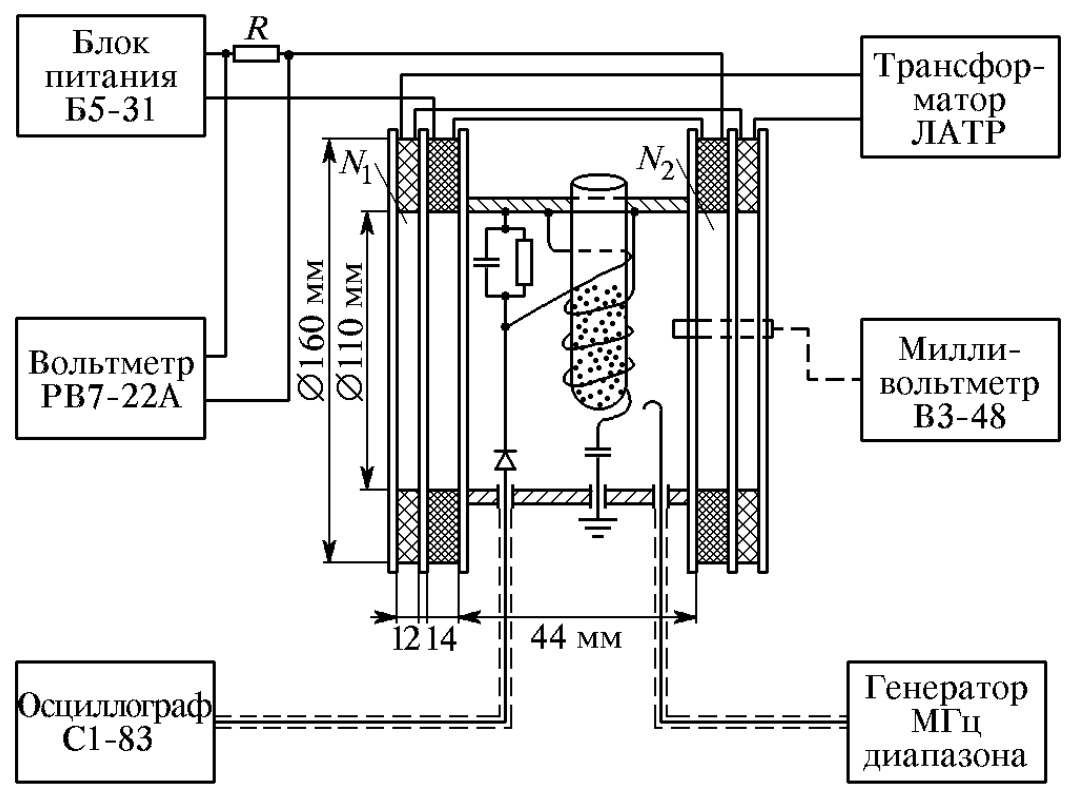
\includegraphics[width=0.5\linewidth]{exp}
			\caption{Схема установки}
		\end{figure}        
		
		Параметры установки: $N_1 = 1500, d_1 = 0.23\,cm, N_2 = 4500, d_2=0.29\,cm$
	\newpage
\begin{multicols}{2}
[
\section{Экспериментальная установка}
]
    Настроим генератор на резонансную частоту колебательного контура, определили значение частоты при максимальном и половинных значениях амплитуды выведенного на осциллограф сигнала:
	
	$f_{0} = 126.76 \, \text{МГц}$
	
	$f_{h} = 126.97 \, \text{МГц}$
	
	$f_{l} = 126.49 \, \text{МГц}$
	
	Рассчитаем добротность
    
    $$ Q = \frac{f}{\Delta f} = \frac{126.76}{0.48} = 264.1 $$
    
    Теперь настроим установку на наблюдение резонансного сигнала. Резонансное поглощение возникает при совпадении в некоторые моменты времени поля $B(t)$ с полем резонансного поглощения на частоте колебательного контура $B_0=\frac{\mathrm{h}f_0}{g\mu_B}$
\end{multicols}

    \begin{figure}[h!]
			\begin{center}
				\begin{minipage}{0.49\linewidth}
					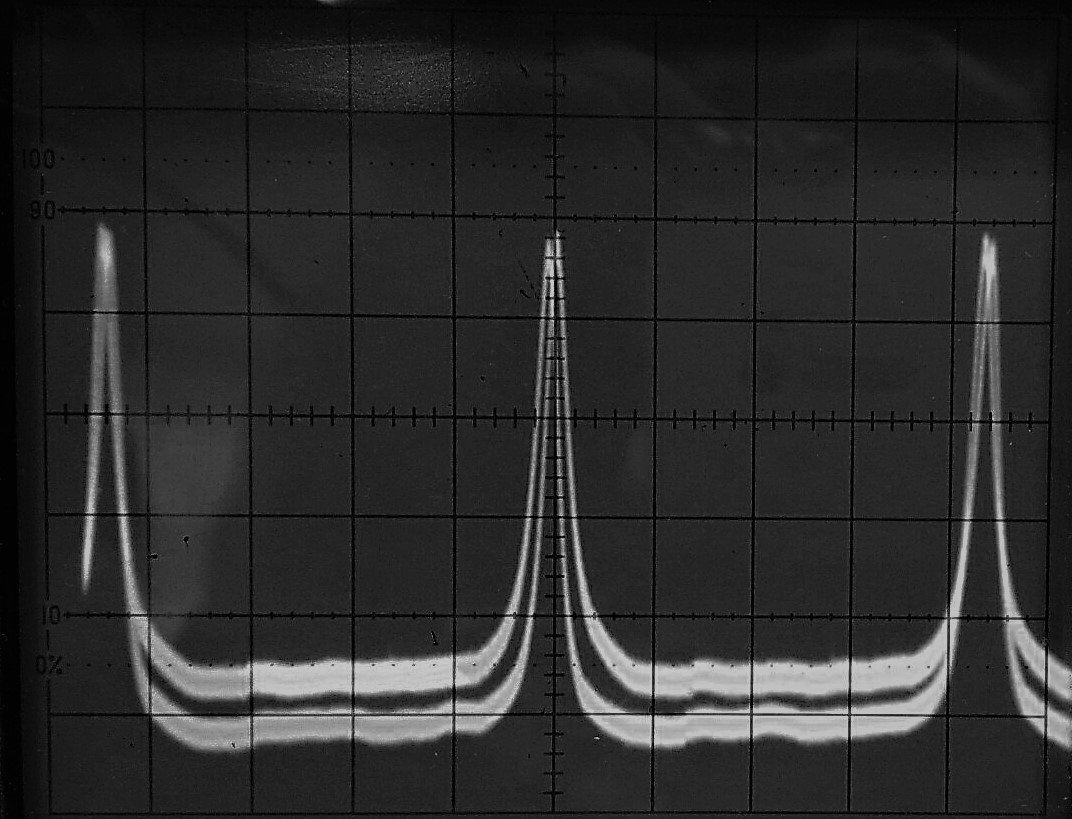
\includegraphics[width=\linewidth]{oscilloscope.jpg}
					\caption{Резонансное поглощение}
				\end{minipage}
				\hfill
				\begin{minipage}{0.49\linewidth}
					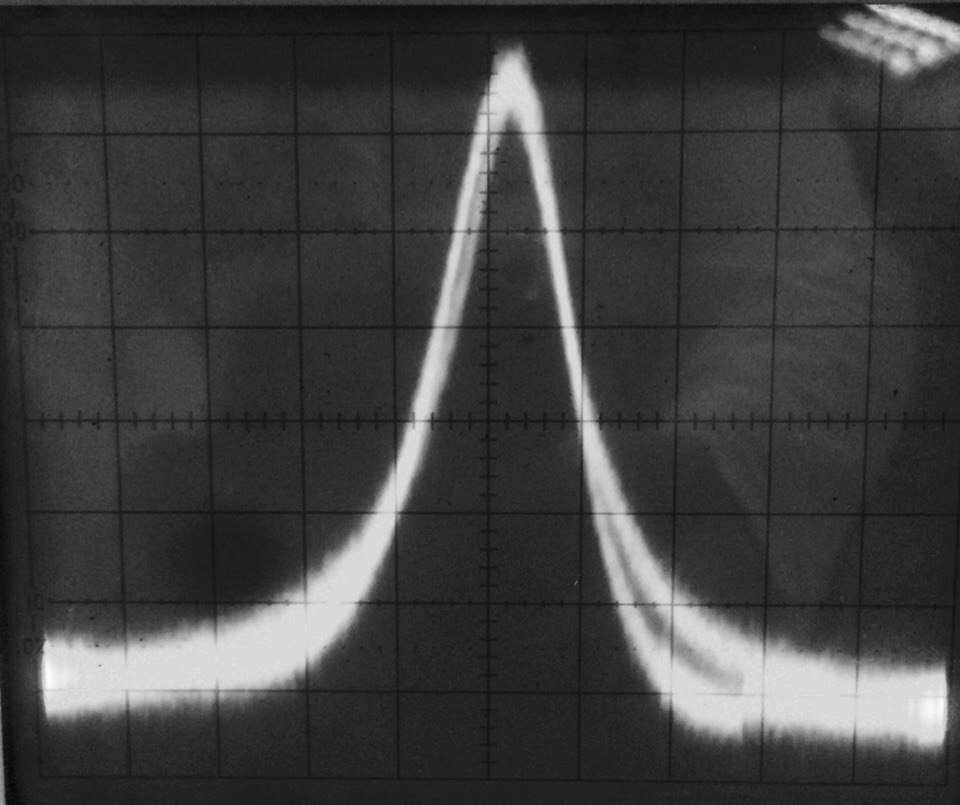
\includegraphics[width=\linewidth]{second.jpg}
				\end{minipage}
			\end{center}
			\caption{Точно настроенный пик}
		\end{figure}

Переменное поле модуляционных катушек наводит в пробной катушке ЭДС индукции,
по которой можно определить величину поля. 
Зная параметры катушки $N_{проб} = 45$, $d = 15.2 \pm 0.1 \; мм$ и ЭДС, определим величину модулирующего поля:


\begin{equation}
B_{мод} = \sqrt{2} \frac{2\varepsilon_i}{\pi^2 d^2N_{проб} \nu} = \sqrt{2} \frac{2 \cdot 2.51 \cdot 10^{-3}\, \text{В}}{\pi^2 \cdot 14.5^2 \cdot 10^{-6} \, \text{м} \cdot 45 \cdot 50\, \text{Гц}}  = 1.52 \cdot 10^{-3} \,\text{Тл} = 1.52 \, \text{мТл}
\end{equation}

тогда для полуширины на полувысоте линии резонансного поглощения (в единицах поля) получим

\begin{equation}
\Delta B  = \frac{A_{1/2}}{A_{\text{полн}}} В_{\text{мод}} = \frac{1}{10.4}\cdot 1.52 = 0.146 \,\text{мТл}  
\end{equation}

Определяем g-фактор. Для этого подаем в основные катушки переменный ток 
), а ЭДС индукции измеряем при помощи пробной катушки. Строим каллиб-
ровочный график:
\begin{figure}
    \centering
    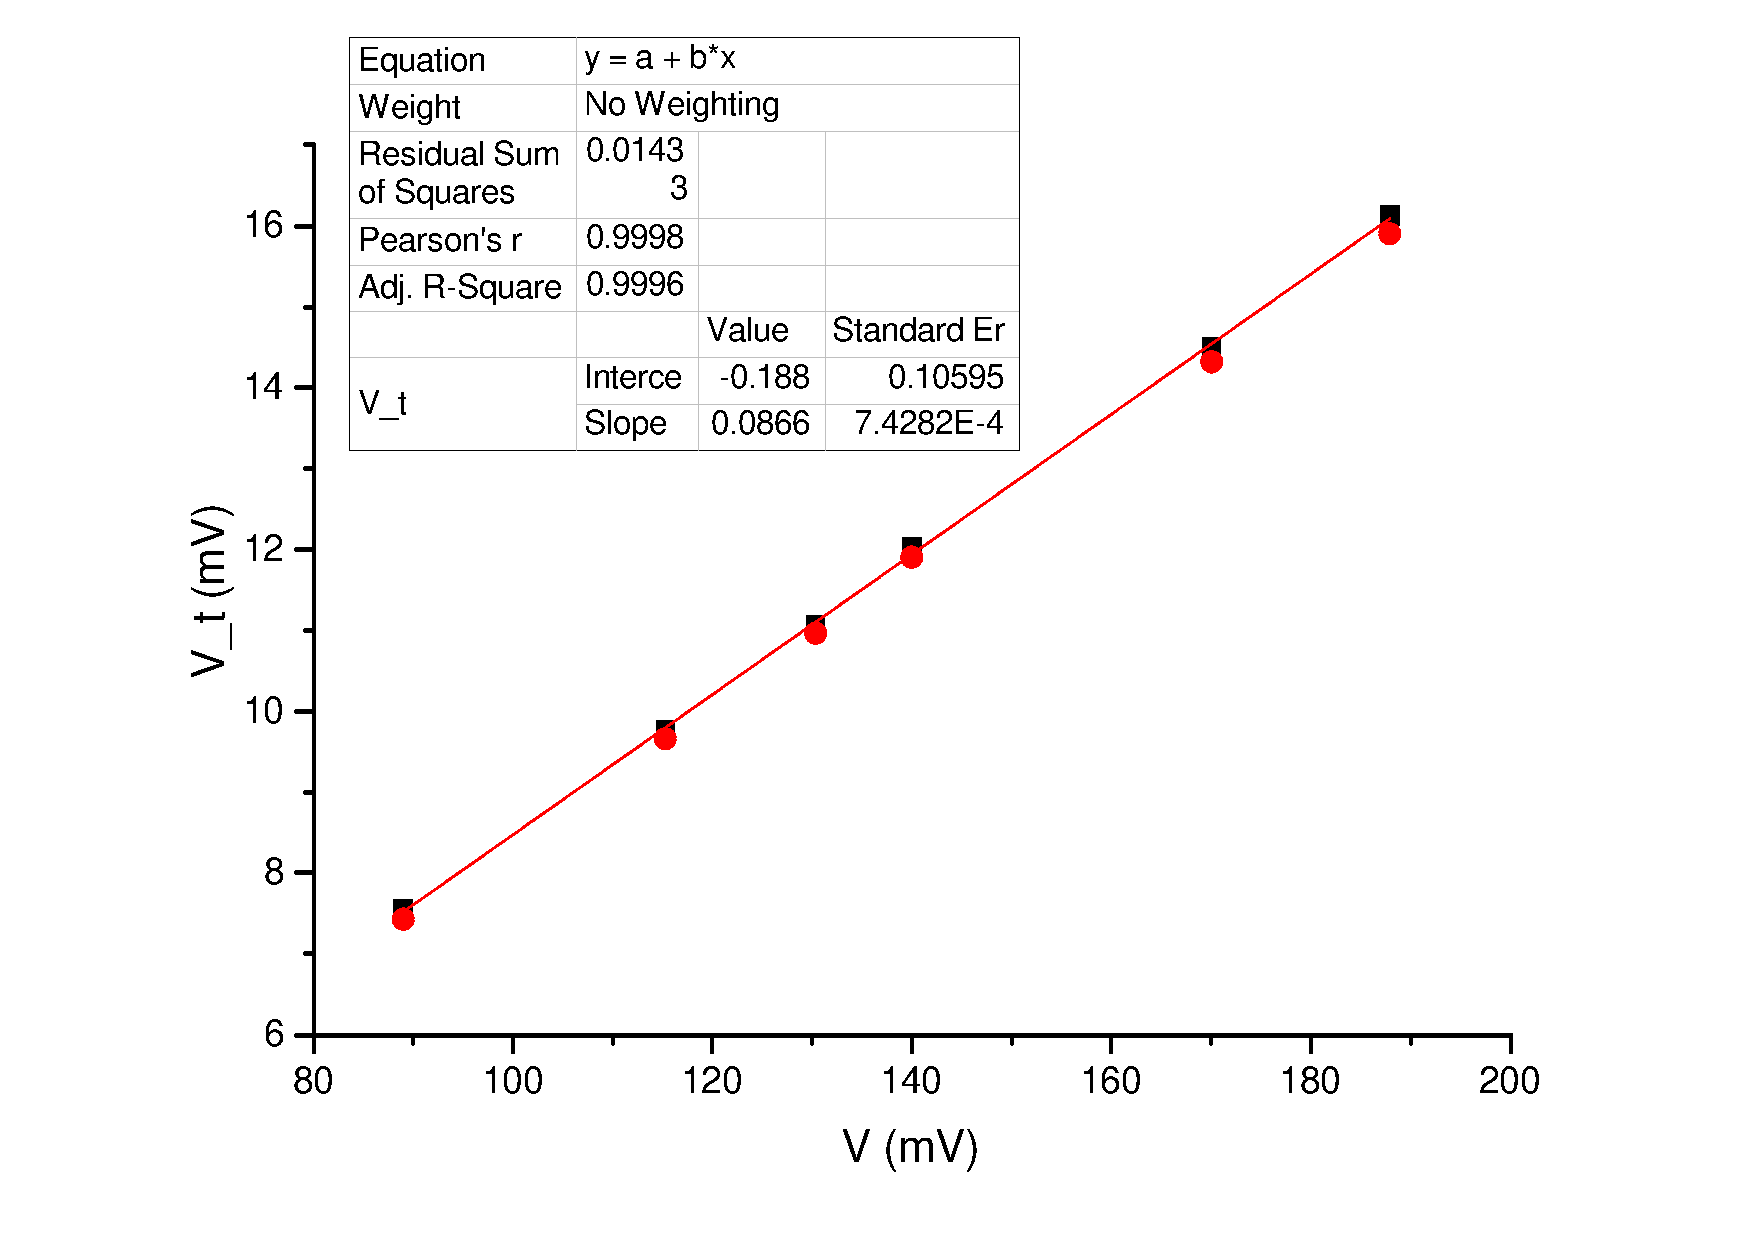
\includegraphics[width = 0.6\linewidth]{cal}
    \caption{ Зависимость ЭДC индукции в пробной катушке от падения напряжения в цепи основных катушек}
    \label{fig:my_label}
\end{figure}
    
    При $V = 122.84\,\mathrm{mV}$ получаем $V_t = 10.45\pm0.08$. Тогда
    \begin{equation}
        B_0 = \frac{V_t}{NS\omega} = 7.03\pm 0.45\,\mathrm{mT}
    \end{equation}
    Отсюда получаем g-фактор равный $g = 1.9\pm 0.2$.
    
    Построим график зависимости резонасной частоты от тока в цепи основных катушек для проверки линейности расщепления уровней.
    
    \begin{figure}[H]
        \centering
        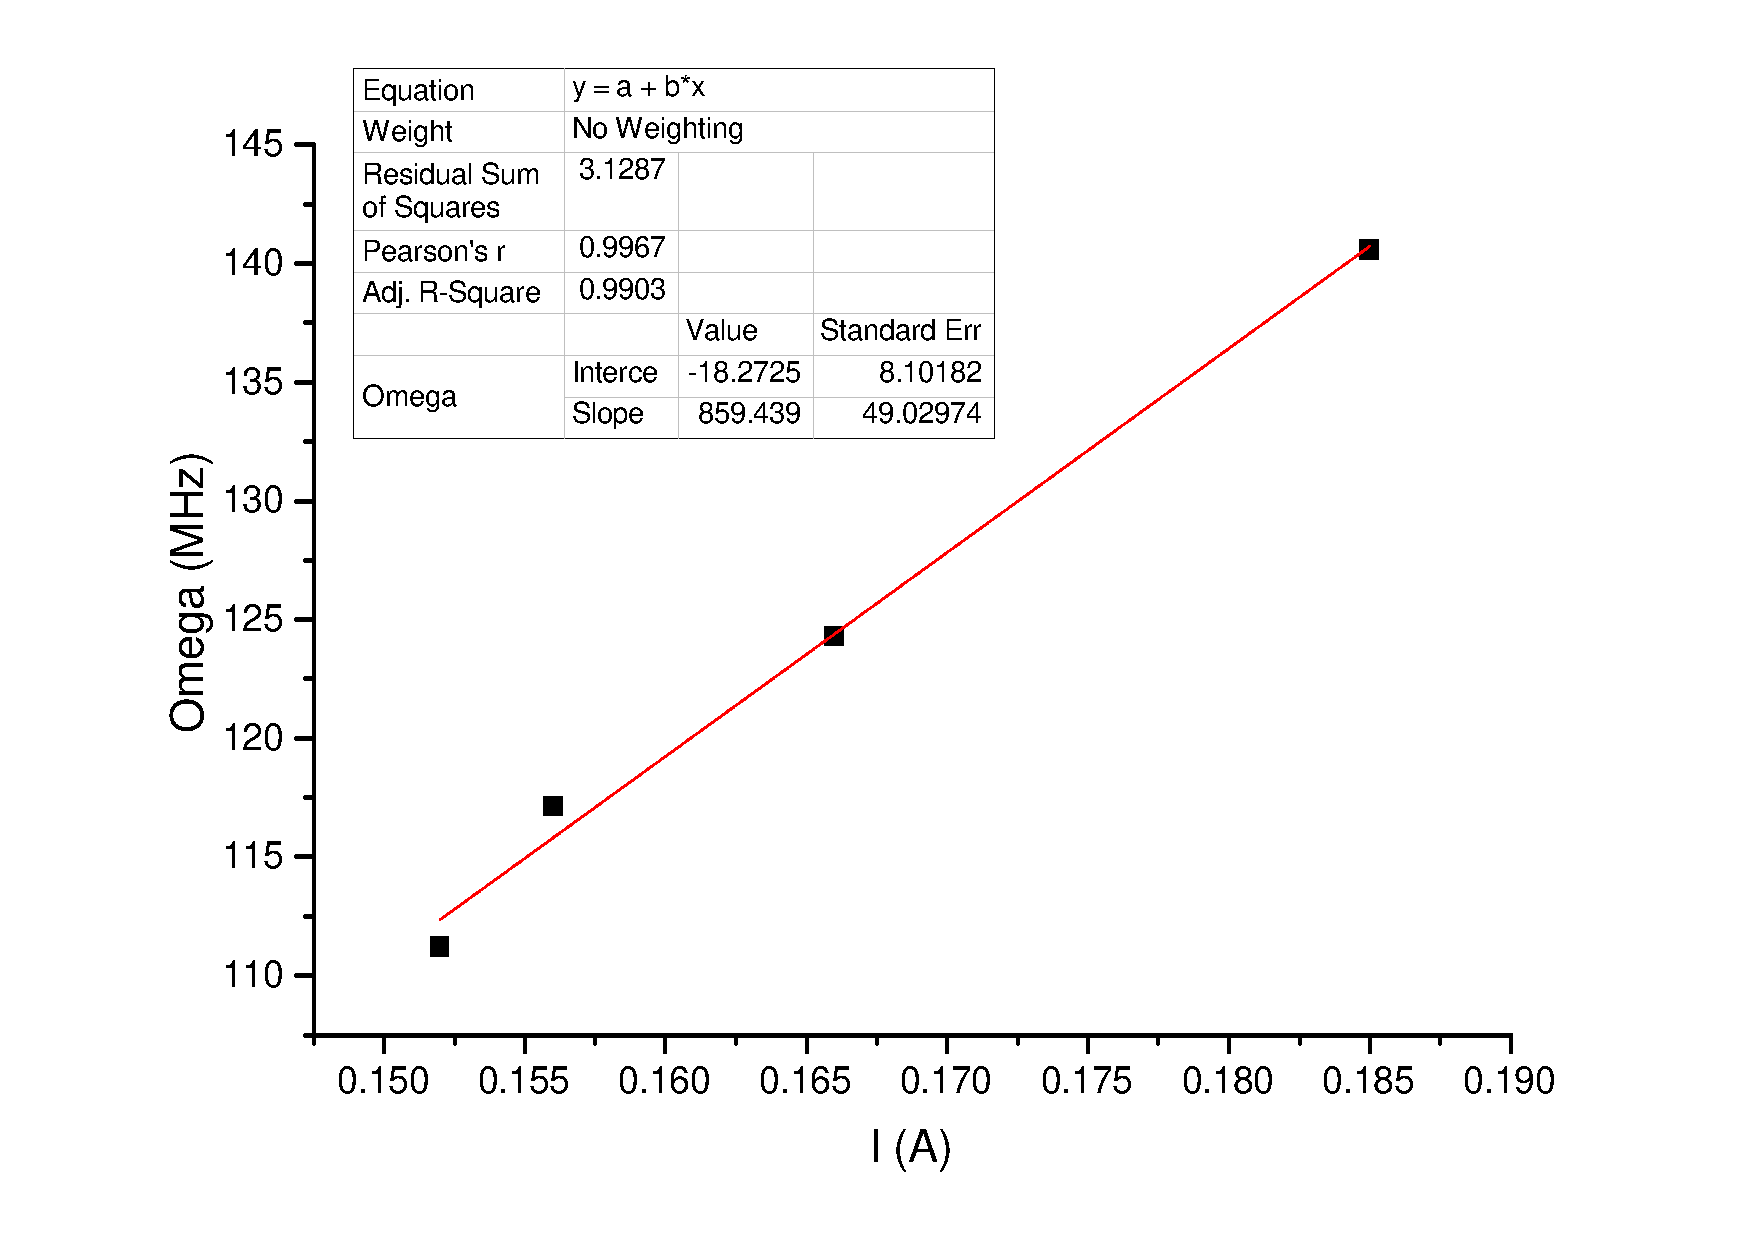
\includegraphics[width = 0.6\linewidth]{lin.pdf}
        \caption{Зависимость резонансной частоты от тока}
    \end{figure}
    
    График, как видно, линейный.
   \section{Вывод}
    Рассчитали $g-$фактор, пусть и за месяц, но рассчитали, кроме того было обнаружено, что зеемановской расщепление линейно по полю.
    

\end{document}